%
%  $Description: The Dissident File System - CMPS221: Advanced Operating Systems.  
%

\documentclass[10pt,twocolumn]{article} 
\usepackage{times,mathptmx,fullpage}
% Allows you to put literal text into your document without having
% LaTeX try to interpret it.
\usepackage{verbatim}
% Sorts citations numerically and "combines" adjacent ones
\usepackage{cite}
% Allows you to individually label subfigures in a multi-part figure
\usepackage{subfigure}
% Allows the definition of macros that are smart about adding space
% after text in a macro
\usepackage{xspace}
\usepackage{graphicx}
\graphicspath{/}

% Redefine the percentage of the page that can be used for floats (figures,
% tables, etc.)
\renewcommand\floatpagefraction{.9}
\renewcommand\dblfloatpagefraction{.9}
\renewcommand\topfraction{.9}
\renewcommand\dbltopfraction{.9}
\renewcommand\bottomfraction{.9}
\renewcommand\textfraction{.1}
\setcounter{totalnumber}{10}
\setcounter{topnumber}{10}
\setcounter{dbltopnumber}{10}
\setcounter{bottomnumber}{10}

% Set values for float separation from text
\setlength{\floatsep}{1.5ex plus1.0ex minus 0.2ex}
\setlength{\dblfloatsep}{1.5ex plus1.0ex minus 0.2ex}
\setlength{\textfloatsep}{1.5ex plus1.0ex minus 0.2ex}
\setlength{\dbltextfloatsep}{1.5ex plus1.0ex minus 0.2ex}
\setlength{\abovecaptionskip}{0.5ex}
\setlength{\belowcaptionskip}{0.5ex}

% Don't allow widows or clubs - single lines at the start/end of a column
\widowpenalty=10000
\clubpenalty=10000

\newcommand{\latex}{\LaTeX\xspace}
\pagestyle{plain}

%------------------------------------------------------------------------- 
\begin{document}

\title{The Dissident File System}

\author{
Aneesh Neelam \\
\textit{Univ. of California, Santa Cruz} \\
\textit{aneelam@ucsc.edu}
}

\maketitle
\thispagestyle{empty}

\begin{abstract}
We present the Dissident Filesystem, a Filesystem in Userspace (FUSE) that combines aspects of steganography and encryption to protect data from untrusted parties. It stores data blocks in plain sight, but individual data blocks are meaningless, requiring a combination of data blocks to obtain the actual data. The filesystem has been developed primarily for GNU/Linux systems. However, it can easily be made to work with any operating system that supports the FUSE API. 
\end{abstract}

%------------------------------------------------------------------------- 
\section{Introduction}

Dissidents may use many tools to protect their digital data, online identity, etc. from an authoritarian government. But these tools have their advantages and disadvantages. Depending on the laws of the State and the legal precedents established, the dissident may be compelled to reveal incriminating data to the State ~\cite{ex2}. Failure to do so can lead to severe fines and imprisonment.  Therefore, it is not enough for the dissident to use the tool to conceal data or identity, but also conceal the use of such a tool from the State. Hence, both encryption and steganography must be applied for this. 

The biggest problem with encryption is that you can not easily hide the fact that you are doing so. If a third party analyzes the data blocks, they may not be able to read the data, but they can conclude that it has been encrypted. They can then ask for the encryption key. In countries such as the United States, you cannot be compelled to reveal anything that incriminates you ~\cite{ex12}. However, not all States have such legal protections.  Unfortunately, there are some which even torture for such information. An encrypted filesystem cannot be read without the decryption key(s), but the State can compel the dissident to decrypt it or share the decryption key(s) ~\cite{ex2,ex10}. 

Steganography is used to hide the presence of a message from a third party ~\cite{ex3}. But, it does not protect the data itself if the presence is known. Hence, just steganography is not a feasible option. Even in chaotic systems, a discernible pattern with limited predictability can be found. Also, by analyzing the size of the data and the content, anomalies will be found and the use of steganography can be detected ~\cite{ex3}. The State can eventually retrieve the dissident’s data from the disk drives. 

The Dissident filesystem employs both encryption and steganography. A data block stored on the Dissident filesystem is split into multiple blocks, each of which does not produce the original data by themselves, but combined they can be used to construct the original data. These blocks can be placed all over the filesystem, and only using a private key can one ascertain which data blocks correspond to which files. It has been implemented using the FUSE API, which is supported by many POSIX systems, including OS X, Linux, and FreeBSD ~\cite{ex1}. 

In the next section, we shall see the approaches that others have taken to solve this problem of safeguarding data while maintaining plausible deniability. In Section III, we shall describe how the Dissident File System is implemented, how it works and how it attempts to solve this problem. In Section IV, we shall talk about the current state of the implementation, and its limitations, and evaluate its performance. We shall then conclude and discuss future work in Section V. 

%------------------------------------------------------------------------- 
\section{Related Work}

A lot of work has been done to protect data stored on disks from third parties. Various encryption algorithms have been devised and implemented in a variety of languages and for many platforms. There are two primary kinds of encryption for data stored on disks: Disk Encryption and Filesystem encryption. 

Disk encryption encrypts the entire disk, including the free space ~\cite{ex4,ex5,ex6}. There are ways to defeat this mechanism, however. It is possible to use a keylogger to capture the key when the user is entering it. Another method is called a cold-boot attack, where the key may be stored in RAM for comparison and since DRAM and SRAM are still readable for a few seconds after the system is shutdown, the contents of the RAM may be dumped and analyzed ~\cite{ex7}. Various mechanisms to speed up disk encryption have been developed. Newer CPU architectures have special AES instructions and specialized hardware for encrypting and decrypting data that is encrypted using the AES algorithm ~\cite{ex8}. 

Filesystem encryption, on the other hand, encrypts files individually in the filesystem layer and stores them. When reading the data back, the filesystem seamlessly decrypts the data. IBM developed Encrypted Filesystem (EFS) for the AIX systems which employs this method to safeguard files stored on disk ~\cite{ex9}. 

Both disk and filesystem level encryption suffer from the same problem: The existence of the data protected using encryption and the use of encryption mechanisms cannot be denied ~\cite{ex2}. 

Steganography has also been employed to safeguard data on disk. The Steganographic File System was developed to give users an element of plausible deniability that encryption alone cannot provide. Users cannot be compelled to divulge the key if the adversary is not aware that the data even exists. The user can confidently deny the existence of the data in such a case ~\cite{ex10}. But, if data hidden using steganography can be found with some level of effort and time. This data is generally not encrypted as that breaks the steganography and subsequently does not offer plausible deniability. 

An encryption tool called Truecrypt was developed that also had a plausible deniability feature. The disk is split into two volumes. One volume contains the actual data, the other contains dummy data that the user is willing to sacrifice. Two keys are used to decrypt the disk. One key only decrypts one of the volumes. Hence, the user can give away the key corresponding to the volume with dummy data, if compelled and the sensitive data in the other volume is still safe ~\cite{ex2}. But, the disk can be carefully analyzed and the size of the volume would not add up to the size of the disk, in which case the adversary can compel the user to disclose the actual key ~\cite{ex11}. 

%------------------------------------------------------------------------- 
\section{Overview and Implementation}

The Dissident File System reconstructs file blocks by combining (N - 1) random blocks, and one particular block to get the original data. Logical XOR is done on the data of the N blocks, to get the actual data the user wants. The random file blocks are chosen based on a private key specified by the user when the filesystem is mounted. Hence, it uses aspects of encryption and steganography. 

Currently, the Dissident File System is implemented using the FUSE API as a stackable filesystem, specifically for Linux systems. This mechanism is developed for individual files, and the performance of the filesystem has been evaluated on a Linux system. However, it can be adapted trivially to work on other POSIX systems that also support the FUSE API. 

Every file that is written to the Dissident File System is split into N separate data buffers which are generated such that the XOR of data of these buffers will give the original data. When the file is to be read back, the filesystem reads these N files and XORs the data to obtain the original file. Without the private key, the filesystem cannot decide which files are related, and which files to XOR to obtain the original data. 

The Dissident File System offers some level of plausible deniability and also protects the data stored on the disk. The presence of (N - 1) random files gives the user the ability to store dummy data that can safely be exposed to the adversary. And without the private key, the adversary cannot quickly ascertain which of the random files are relevant to reading a particular file. However, the current implementation has certain limitations, and many challenges still need to be addressed that we shall describe in the next section. 

%------------------------------------------------------------------------- 
\section{Evaluation}

In this section, we evaluate the performance of the Dissident File System and also describe some of its limitations and various implementation challenges that we faced. 

\subsection{Performance}
We ran experiments to gauge the performance of the current implementation of the Dissident File System. We used dd, a command-line utility for Unix that can be used to benchmark drive performance. We used dd to evaluate the read and write performance of files on the Dissident File System and the Linux ext4 filesystem as a basis for comparison. 

We also timed copying large files from the Dissident File System volume to the Linux ext4 filesystem volume and back, and between two Dissident File System volumes and between two ext4 volumes as a basis for comparison. 

All experiments were done on the same Linux virtual machine, with the same configuration and on the same physical hardware. 


\begin{figure}[thpb]
  \centering
  	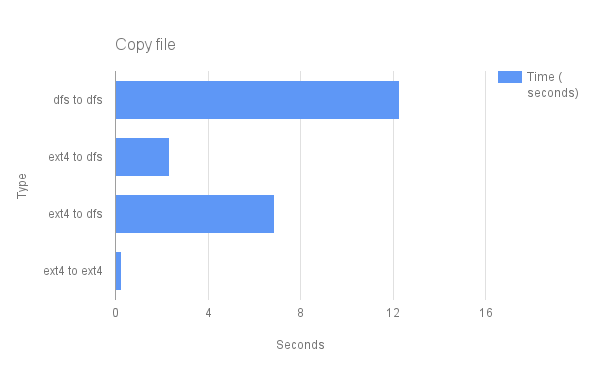
\includegraphics[width=\columnwidth]{cp}
    \caption{Copying a 241938432 bytes file between volumes, using time and cp UNIX utilities. Less is better performance here. dfs here is the Dissident File System. }
	\label{fig:cp}
\end{figure}

\begin{figure}[thpb]
  \centering
  	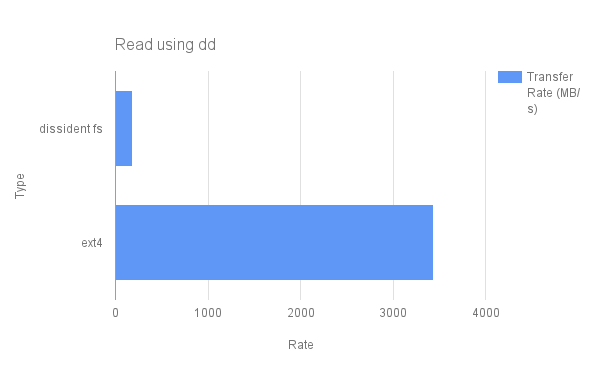
\includegraphics[width=\columnwidth]{dd_read}
    \caption{Reading a 409600000 bytes file, using time and dd UNIX utilities. More is better performance here.}
	\label{fig:ddread}
\end{figure}

\begin{figure}[thpb]
  \centering
  	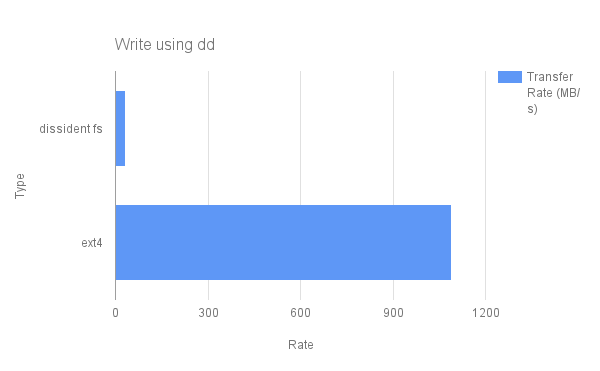
\includegraphics[width=\columnwidth]{dd_write}
    \caption{Writing 409600000 bytes to a file, using time and dd UNIX utilities. More is better performance here.}
	\label{fig:ddwrite}
\end{figure}

As you can see, the performance is severely degraded, as expected on the Dissident File System when compared with a more general filesystem like ext4. 

\subsection{Limitations}

The current implementation has certain limitations that still need to be addressed. The (N - 1) random file buffers are still not generated arbitrarily. Due to the nature of XOR, it is still possible to ascertain which of these correspond to which file. Also, if there is only a single file stored on the volume, it is trivial to determine the other random files. Generating data such that meaningful data is obtained when XORed with specific files is one of the greatest challenges in this project, and there is still work to be done to perfect this technique. 

Due to this, the disk can be analyzed carefully, and a skilled adversary with some effort and time might be able to conclude that some form of encryption has been used to protect data. The disclosure of the private key used by the Dissident File System could be compelled by the adversary, actually defeating the filesystem. 

Due to the nature of how the filesystem has been conceived, disk space is wasted for this purpose. Every file would take up N-times their original size on the Dissident File System. Reading and writing every file would actually entail reading and writing N different files, which severely hinders performance. It is a tradeoff between plausible deniability and data protection versus efficiency and performance. 

%------------------------------------------------------------------------- 
\section{Conclusion}

The Dissident File System uses aspects of steganography and encryption to achieve plausible deniability and to also protect the data. Blocks are placed all over the filesystem and the original data is never stored plainly in any one of them. The location of the blocks is ascertained using a private key. 

The concept and the implementation can be improved upon to combat the severe performance degradation and also make it more reliable and secure. The current implementation is not very efficient, perhaps the reading and writing of the N blocks could be made concurrent, enabling parallelism. This will greatly improve performance, especially on flash-based persistent storage devices like Solid State Drives. 

Currently, the Dissident File System is implemented as a stackable filesystem. This is to quickly have a prototype that makes use of the idea, rather than to spend time and effort designing the filesystem. In the future it can be implemented as an independent filesystem that can be used directly on any device or file. 

%------------------------------------------------------------------------- 
\bibliographystyle{latex8}
\bibliography{latex8}

\end{document}
